\part{The backend}\label{part:nstar}


\chapter{Introduction}\label{chap:nstar-abstract}

Assembly languages are the lowest level of humanly-possible programming there exists nowadays. They were used back in the days for very performance-critical tasks, or even just for fun, as there weren't many other programming languages available. Nowadays, with all the existing ones, most people have never used any assembly language.

Despite their apparent simplicity, and the small amount of work you need to put into creating assembly languages, those are in fact very hard to use. At that low level, there is no such thing as Java's exceptions keeping you from doing dumb things, Rust's linear types keeping you from leaking memory nor even Garbage Collectors. The nice things preventing you from having segfaults simply do not exist, and you are expected to either provide all those things yourself (creating a language runtime) or be very careful about what you are doing each time you write a single instruction (even a simple \texttt{mov} can have undesirable side-effects).

Doing dumb things is something that we must prevent directly when using the language. That way, we do not need to rely on external verification tools or debuggers, trying to know why a program segfaults at a specific point.
This is where a type system can become handy. Typed assembly languages are assembly languages augmented with simple yet powerful type system. Among the most famous typed assembly languages are TALx86~\cite{TALx86} and DTAL~\cite{DTAL}.

TALx86 is basically NASM with a type system, targetting only the x86 architecture. DTAL is much more complicated and embeds a completely dependent type system.

\vspace{\baselineskip}

N*'s goal is to assist users with a simple but powerful type system, as well as other features like what I call ``branch-checking'' which prevents from leaking the control flow of the program, and thus makes a part of the type-checking process meaningful.
But before even being a usable programming language, N* aims at being a compiler backend (much like for example LLVM), and is used as is in the Zilch project. Differences with other compiler backends are mostly the type-system, allowing the compilation of Zilch source code into type-safe instructions.

\vspace{\baselineskip}

Because N* supports compiling to multiple architectures, using different grammars, describing N* will at first be platform-agnostic, treating common aspects between all CPU architectures, and then will be divided into multiple categories, explaining in more details some features on a per-architecture basis\footnote{Note that the target executable format (ELF, PE, \ldots) is also considered as an architecture-specific thing.}.


\chapter{Target: ELF x86/amd64}\label{chap:elfx86amd64}

The first target of N* is the ELF executable file format, for either x86 or amd64 (amd64 is simply an extension of x86 for 64-bits architectures).

\section{Data section}\label{sec:elf86amd64-data}

The \texttt{data} section in N* is the section where you can bind any value to an address (refered to by a label) that will be used during runtime.
This is most commonly done for static data.

\subsection{Grammar}\label{subsec:elf86amd64-data-grammar}

\begin{figure}[h]
  \centering
  \scalebox{.5}{
    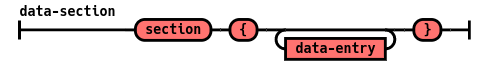
\includegraphics{elf86-amd64-data-grammar-data-section}
  }
\end{figure}
